\documentclass[14pt,a4]{article}

\usepackage{xcolor}
\usepackage{amsmath}
\usepackage{amsfonts}
\usepackage{enumitem}
\usepackage{graphicx}
\usepackage{subcaption}
\usepackage{xepersian}

\settextfont{XB Kayhan}
\setlatintextfont{Times Newer Roman}
\setlatinsansfont{Times Newer Roman}

\title{\vspace{-4cm} \textbf{پاسخ تمرینات سری اول درس شناسایی آماری الگو}}
\author{محمدرضا غفرانی  ۴۰۰۱۳۱۰۷۶}
\date{\today}

\begin{document}

\maketitle

\section*{سوال یک}

\subsection*{قسمت الف}

مسئله را می‌توان هم به شکل یک مسئله‌ رگرسیون و هم می‌توان به شکل مسئله‌ کلاس‌بندی حل کرد.
اگر بخواهیم مسئله را به شیوه‌ رگرسیون حل کنیم باید سن فرد را به صورت پیوسته
در نظر گرفته و پس از پیش‌بینی دقیق سن بررسی کنیم آیا این سن در بازه‌ی ۷ تا ۱۴ سال قرار
دارد یا خیر. اما اگر بخواهیم مسئله را به شکل کلاس‌بندی حل کنیم مدل باید بررسی کند که آیا سن
فرد در بازه ۷ تا ۱۴ سال قرار دارد. مدل پیشنهادی ما مسئله را به شکل کلاس‌بندی حل می‌کند.

\subsection*{قسمت ب}

سنسور وزن، سنسور قد، سنسور صدا، جنسیت

\subsection*{قسمت ج}

از افراد مختلفی که سن‌ آن‌ها در بازه‌ی ۷ تا ۱۴ سال قرار دارد و همچنین افرادی را که
سن آن‌ها در این بازه نیست، نمونه جمع‌آوری می‌کنیم. برای هر فرد ویژگی‌های
قد، وزن، فرکانس صدا و جنسیت جمع‌آوری می‌شود.‌

\subsection*{قسمت د}

با توجه به آن که جامعه‌ هدف اغلب کودکان و نوجوانان هستند، بنابراین با تاسیس
یک باجه در پارک اقدام به جمع‌آوری ویژگی‌های مدنظر از افراد می‌کنیم. البته این اقدام به
صورت داوطلبانه و با موافقت والدین جمع‌آوری می‌شود.

\subsection*{قسمت ه}

قد، وزن، فرکانس صدا و جنسیت

\subsection*{قسمت و}

با توجه به آن که ممکن است مقیاس بعضی از ویژگی‌ها با دیگران تفاوت داشته باشد و این امر
باعث اختلال در فرآیند آموزش شود، بنابراین همه‌ی ویژگی‌ها را به بازه‌ $[0,1]$ مقیاس می‌کنیم.

\subsection*{قسمت ز}

ما ویژگی فرکانس صدا را به عنوان یک ویژگی در نظر گرفته‌ایم. این ویژگی در هنگام آموزش مشکلی
ایجاد نمی‌کند اما اندازه‌گیری آن در هنگام عملیاتی کردن سیستم از این جهت دشوار است که
شهر‌بازی جای شلوغی است در نتیجه باید صدای فرد از دیگر صدا‌ها تفکیک شود.

\subsection*{قسمت ح}

از آن جا که علاوه بر ویژگی قد، ویژگی‌های دیگری را نیز برای تشخیص بازه‌ی سنی فرد به کار برده‌ایم،
در نتیجه دقت تشخیص ما بهبود خواهد یافت. اما مشکلی که سیستم فعلی دارد، استفاده از سنسور‌های مختلف
است. این کار فرآیند تشخیص سن را طولانی کرده و باعث تشکیل صف‌های طولانی و در نتیجه کاهش رضایت‌مندی
می‌شود.

\section*{سوال دو}

ویژگی‌های زیر برای اهدافی که در صورت سوال بیان شده است، پیشنهاد می‌شود.

\begin{itemize}
    \item \textbf{شناسایی اثر انگشت:} اثر انگشت فرد را همانند تصویر \ref{fingerprint}
    به ناحیه‌هایی تقسیم می‌کنیم. برای هر یک از این ناحیه‌ها دو ویژگی (۱) حداکثر تعداد تلاقی خط عمودی رسم شده
    با خطوط موجود در آن ناحیه، (۲) حداکثر تعداد تلاقی خط افقی رسم شده با خطوط موجود در آن ناحیه و
    (۳) شیب میانگین خطوط موجود در آن ناحیه را به عنوان ویژگی‌های بیان کننده آن ناحیه در نظر می‌گیریم.
    در نهایت با استفاده از ویژگی‌های مربوط به هر ناحیه یک ماتریس برای کل اثر انگشت
    تشکیل داده و مسئله را حل می‌کنیم.

    \begin{figure}[h]
        \centering
        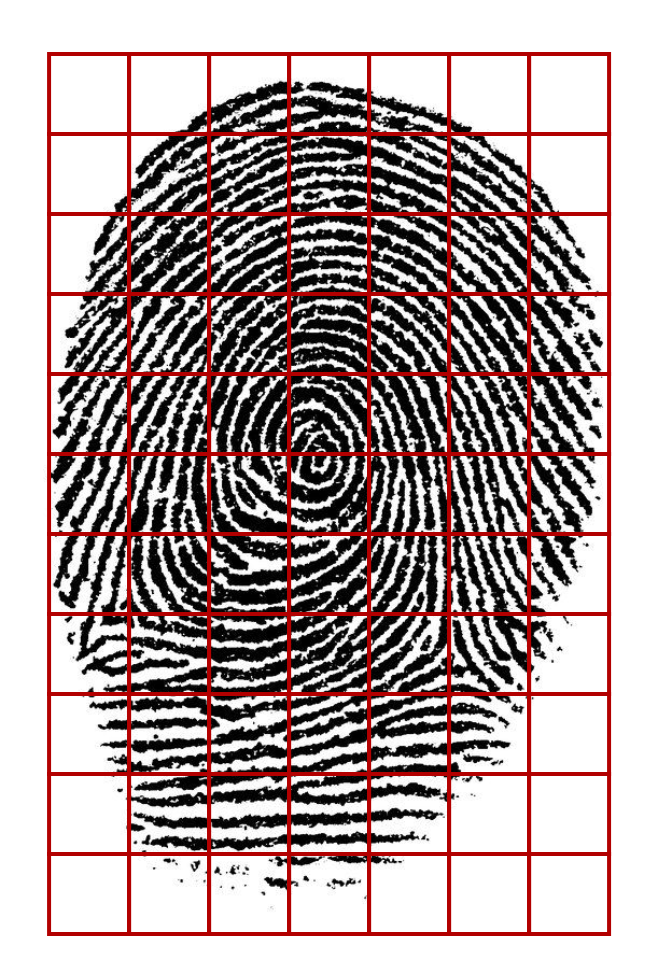
\includegraphics[scale=0.4]{images/q2/fingerprint.png}
        \caption{ناحیه‌بندی اثر انگشت}
        \label{fingerprint}
    \end{figure}

    \item \textbf{شناسایی احساس:} برای شناسایی حالت از سه ویژگی حالت ابرو، حالت چشم و حالت لب کمک می‌گیریم.
    ابرو را با یک خط مدل می‌کنیم. این خط می‌تواند شیب مثبت (ابرو رو به پایین)، منفی (ابرو رو به بالا)
    و صفر (ابرو افقی) داشته باشد. برای چشم دو حالت کاملا باز و باز را در نظر می‌گیریم. برای لب نیز مشابه
    چشم دو حالت گرد، افقی، نیم‌دایره رو به بالا و نیم‌دایره رو به پایین در نظر می‌گیریم.
    با استفاده از این مدل سعی می‌کنیم حالت‌های مختلف چهره را بیان کنیم. برای مثال حالت متعجب را
    با حالت‌های لب گرد، چشم‌های کاملا باز و ابرو رو به بالا مدل می‌کنیم.
    \item \textbf{شناسایی مشی\LTRfootnote{Gait Recognition}:} برای شناسایی مشی دو ویژگی را
    پیشنهاد می‌کنیم: (۱) نسبت طول فرد در حالت راه رفتن به زمانی که راست ایستاده است و
    (۲) زاویه فرد نسبت به خط عمود بر سطح در سه بعد.
    \item \textbf{شناسایی فعالیت\LTRfootnote{Activity Recognition}:} برای تفکیک کردن وظایف گفته شده
    همانند شکل موجود در سوال و با استفاده از یک دوربین، با استفاده از سرعت حرکت موجود بین سه حالت
    «ایستاده»، «در حال راه رفتن» و «در حال دویدن» تمایز قائل می‌شویم. برای تفکیک وظایف «در حال مطالعه»،
    «در حال دست‌دهی» و «در حال نوشیدن» نیز از زاویه‌ی دست نسبت به خط افقی کمک می‌گیریم. اگر زاویه
    صفر تا ۲۰ درجه باشد، فرد در حالت «دست‌دهی» است؛ اگر زاویه بین ۲۰ تا ۷۰ درجه باشد، فرد در حالت «مطالعه» است؛
    در نهایت اگر زاویه بیشتر از ۷۰ و کمتر از ۹۰ درجه باشد، فرد در حال «نوشیدن» است.
\end{itemize}

در ادامه ویژگی‌هایی برای هر بخش جدا کردن اشیا گفته شده پیشنهاد می‌دهیم.

\begin{itemize}
    \item \textbf{دایره و مربع:} تصویر را مانند شکل زیر سیاه و سفید را به ماتریس تبدیل می‌کنیم.(شکل \ref{circle-and-square-recongition})
    خانه‌هایی از ماتریس که شامل خط سیاه‌رنگ هستند را با عدد یک و باقی خانه‌ها را با عدد صفر نمایش می‌دهیم.
    (در حالت کلی می‌توان هر خانه را با میزان خاکستری بودن آن نمایش داد.)

    \begin{figure}[h]
        \centering
        \begin{subfigure}{0.45\textwidth}
            \centering
            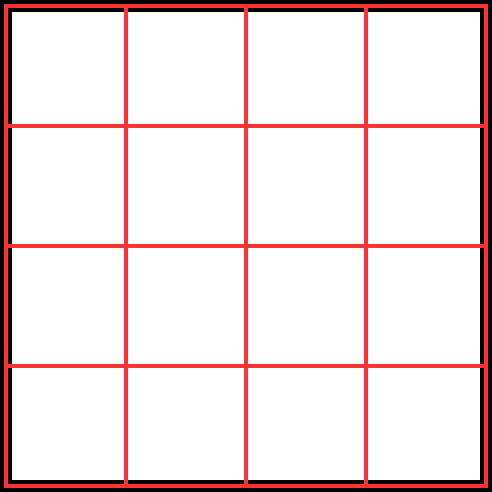
\includegraphics[scale=0.5]{images/q2/square.png}
        \end{subfigure}
        \hfill
        \begin{subfigure}{0.45\textwidth}
            \centering
            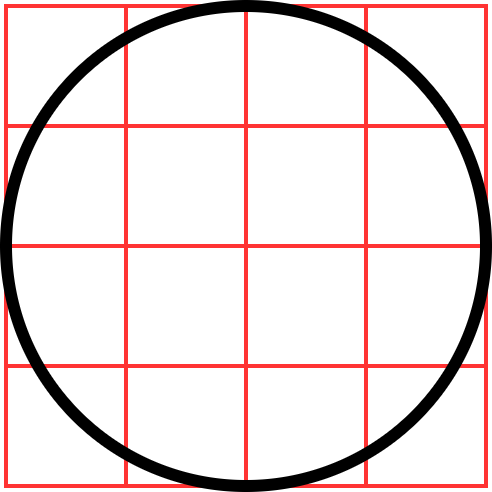
\includegraphics[scale=0.5]{images/q2/circle.png}
        \end{subfigure}
        \caption{مدل‌سازی برای شناسایی مربع و دایره}
        \label{circle-and-square-recongition}
    \end{figure}

    برای مثال در زیر یک نمونه از مربع و دایره مدل شده
    در این مدل آورده شده است.

    \[
        \text{\lr{Circle}} = \left[ \begin{array}{cccc}
        1 & 1 & 1 & 1 \\
        1 & 0 & 0 & 1 \\
        1 & 0 & 0 & 1 \\
        1 & 1 & 1 & 1 \\
        \end{array} \right]
        \hspace{2cm}
        \text{\lr{Square}} = \left[ \begin{array}{cccc}
        0 & 0 & 0 & 0 \\
        0 & 0 & 0 & 0 \\
        0 & 0 & 0 & 0 \\
        0 & 0 & 0 & 0 \\
        \end{array} \right]
    \]

    با تعریف ماتریس مرجع به شکل زیر و مقایسه‌ تفاضل ماتریس شکلی که می‌خواهیم شناسایی کنیم با تفاضل
    ماتریس  متناظر مربع و دایره از ماتریس مرجع شکل مربوطه را شناسایی می‌کنیم.

    \[
        U = \left[ \begin{array}{cccc}
        1 & 1 & 1 & 1 \\
        1 & 1 & 1 & 1 \\
        1 & 1 & 1 & 1 \\
        1 & 1 & 1 & 1 \\
        \end{array} \right]
    \]

    \item \textbf{مربع و مثلث:} تعداد ضلع و مجموع درجه‌های داخلی شکل.
    \item \textbf{شناسایی مثلث با هر ابعاد:} تعداد ضلع باید برابر سه باشد و مجموع زوایای داخلی برابر ۱۸۰ باشد.
    \item \textbf{شناسایی دایره با هر ابعادی:} مشابه روش پیشنهاد شده برای تفکیک «دایره و مربع» عمل می‌کنیم.
    با این تفاوت که ابتدا عکس دریافتی را به یک ابعاد مشخص مقیاس می‌کنیم و سپس مشابه روش گفته شده پیش می‌رویم.
    \item \textbf{مربع با هر دورانی:} داشتن چهار ضلع مساوی و داشتن مجموع زوایای داخلی ۳۶۰ درجه. به علاوه با
    دوران دادن عکس دریافتی می‌توان مشابه روش پیشنهادی برای تفکیک مربع و دایره عمل کرد.
    \item \textbf{تفکیک دایره، مربع و مثلث:} با ارائه ماتریس مثلث به شکل زیر، مشابه روش ارائه شده برای
    تفکیک دایره و مربع عمل می‌کنیم.

    \[
        \text{\lr{Triangle}} = \left[ \begin{array}{cccc}
        0 & 0 & 1 & 1 \\
        1 & 1 & 0 & 1 \\
        1 & 1 & 0 & 1 \\
        0 & 0 & 1 & 1 \\
        \end{array} \right]
    \]

    ماتریس بالا بر اساس شکل زیر رسم شده است.(شکل \ref{triangle-recongition})

    \begin{figure}[h]
        \centering
        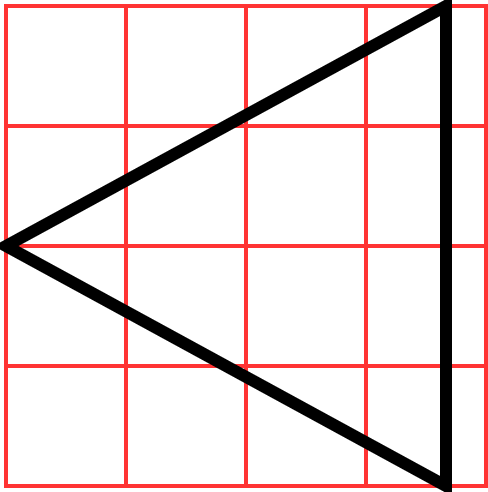
\includegraphics[scale=0.5]{images/q2/triangle.png}
        \caption{مدل‌سازی برای شناسایی مثلث}
        \label{triangle-recongition}
    \end{figure}

\end{itemize}

\section*{سوال سه}

\subsection*{قسمت الف}

نمودار‌های مربوط به این قسمت در شکل \ref{image-for-question1-part1} رسم شده است.

\begin{figure}[h]
    \centering
    \begin{subfigure}{0.32\linewidth}
        \centering
        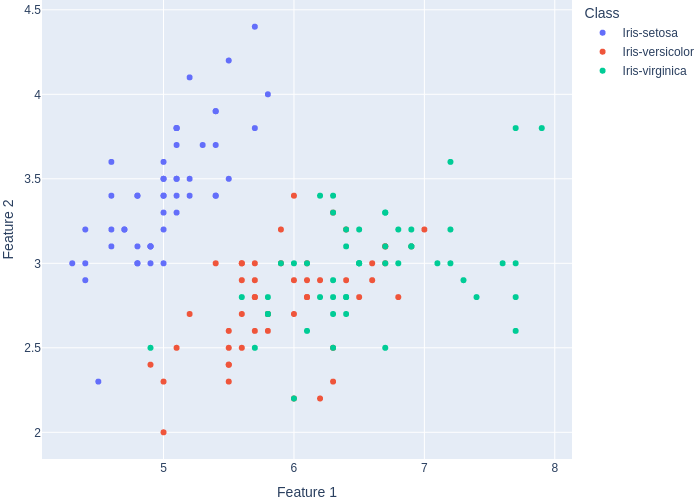
\includegraphics[width=\linewidth]{images/q3/p1/12.png}
    \end{subfigure}
    \hfill
    \begin{subfigure}{0.32\linewidth}
        \centering
        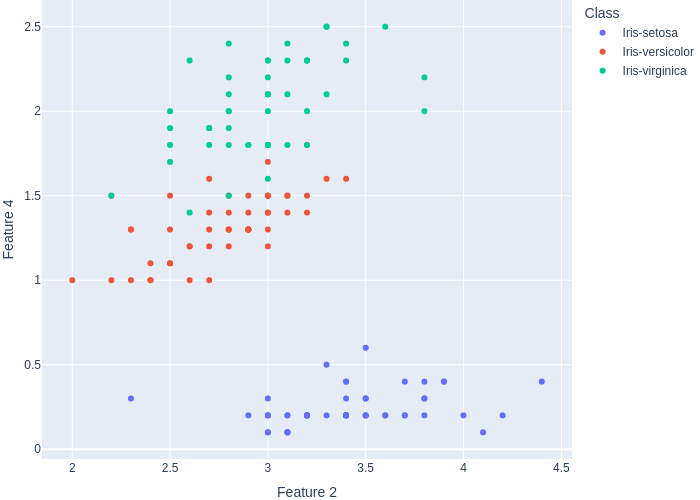
\includegraphics[width=\linewidth]{images/q3/p1/24.png}
    \end{subfigure}
    \hfill
    \begin{subfigure}{0.32\linewidth}
        \centering
        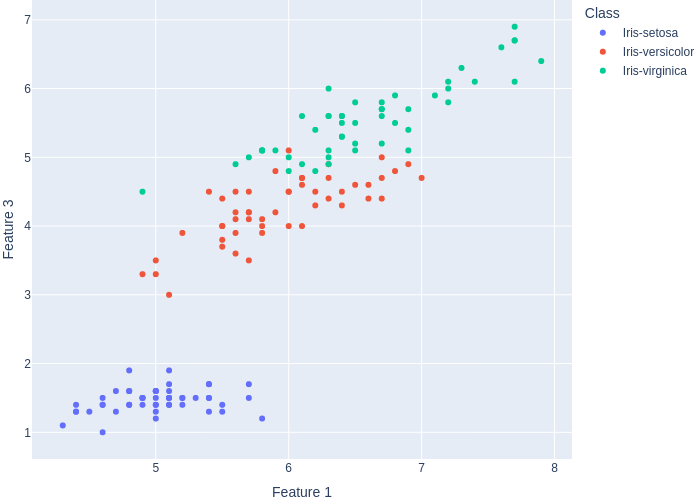
\includegraphics[width=\linewidth]{images/q3/p1/13.png}
    \end{subfigure}
    \caption{شکل سوال سه قسمت الف}
    \label{image-for-question1-part1}
\end{figure}

\subsection*{قسمت ب}

اشکال رسم‌شده با استفاده از تبدیل‌های داده شده در شکل \ref{image-for-question1-part2} مشاهده می‌شود.

\begin{figure}[h]
    \centering
    \begin{subfigure}{0.32\linewidth}
        \centering
        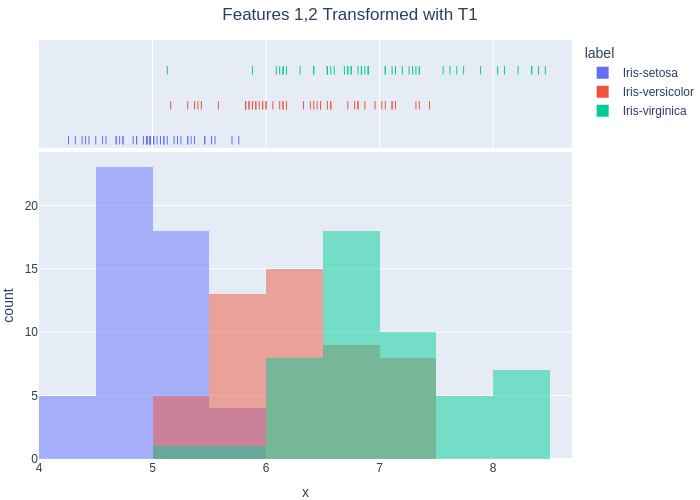
\includegraphics[width=\linewidth]{images/q3/p2/12T1.png}
    \end{subfigure}
    \hfill
    \begin{subfigure}{0.32\linewidth}
        \centering
        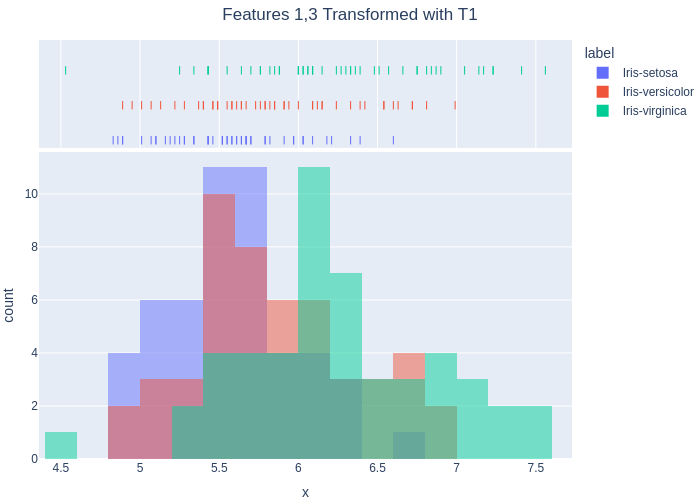
\includegraphics[width=\linewidth]{images/q3/p2/13T1.png}
    \end{subfigure}
    \hfill
    \begin{subfigure}{0.32\linewidth}
        \centering
        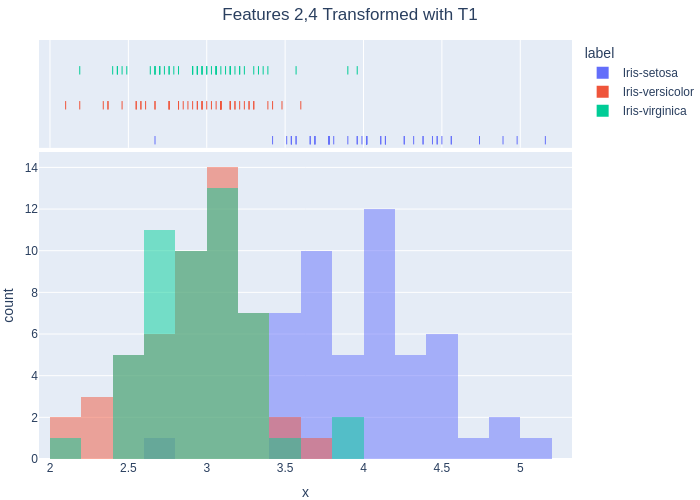
\includegraphics[width=\linewidth]{images/q3/p2/24T1.png}
    \end{subfigure}
    \newline
    \begin{subfigure}{0.32\linewidth}
        \centering
        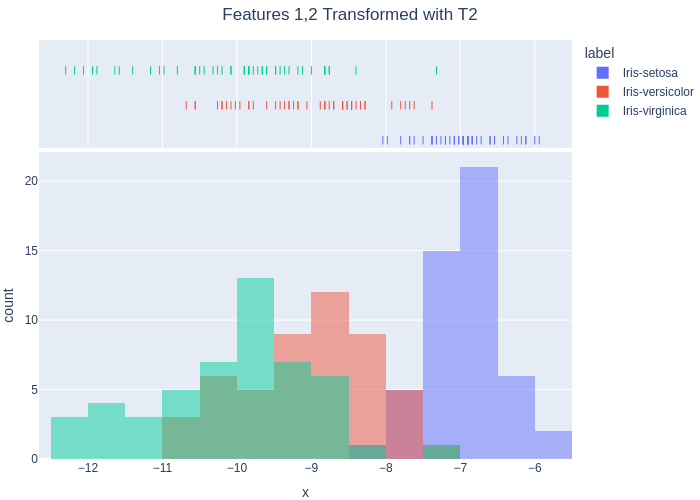
\includegraphics[width=\linewidth]{images/q3/p2/12T2.png}
    \end{subfigure}
    \hfill
    \begin{subfigure}{0.32\linewidth}
        \centering
        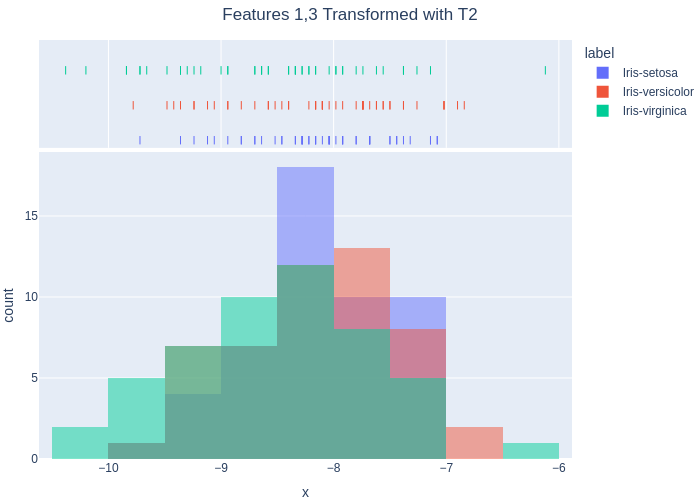
\includegraphics[width=\linewidth]{images/q3/p2/13T2.png}
    \end{subfigure}
    \hfill
    \begin{subfigure}{0.32\linewidth}
        \centering
        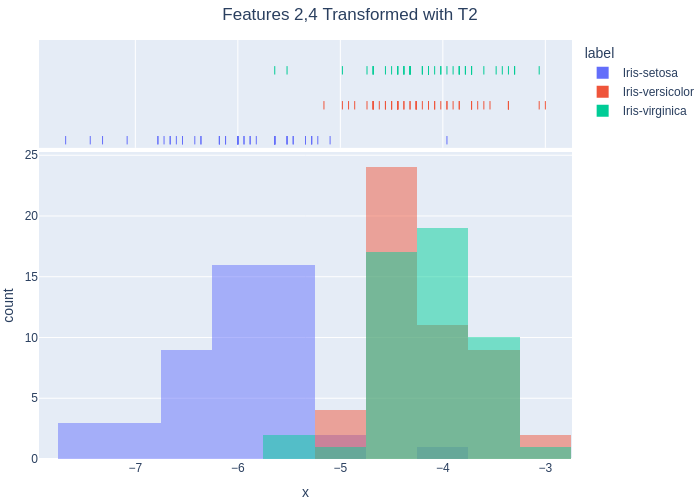
\includegraphics[width=\linewidth]{images/q3/p2/24T2.png}
    \end{subfigure}
    \newline
    \begin{subfigure}{0.32\linewidth}
        \centering
        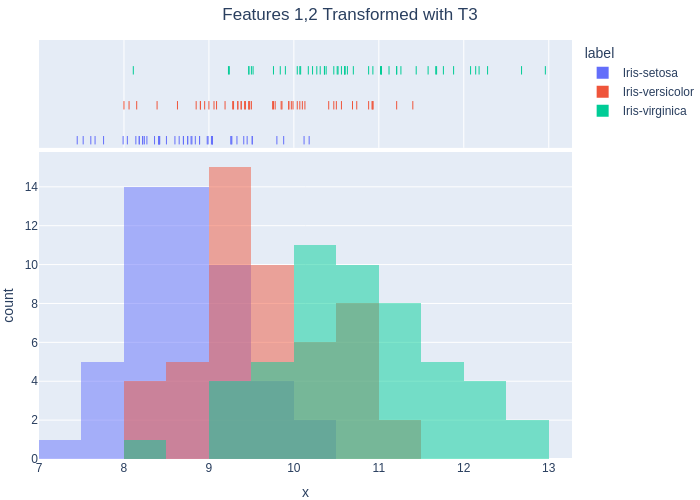
\includegraphics[width=\linewidth]{images/q3/p2/12T3.png}
    \end{subfigure}
    \hfill
    \begin{subfigure}{0.32\linewidth}
        \centering
        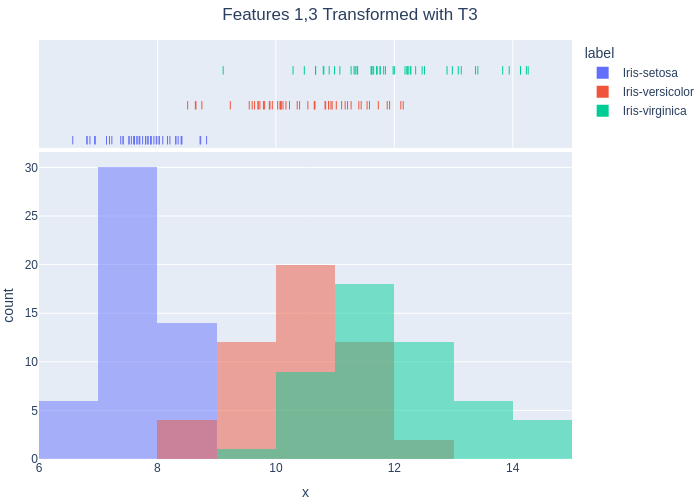
\includegraphics[width=\linewidth]{images/q3/p2/13T3.png}
    \end{subfigure}
    \hfill
    \begin{subfigure}{0.32\linewidth}
        \centering
        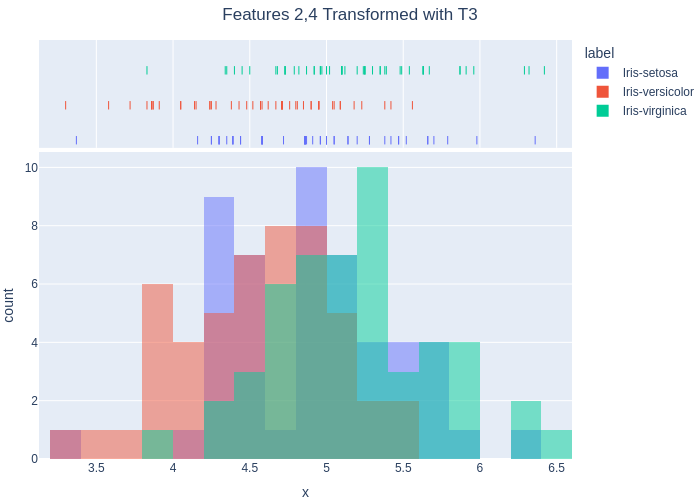
\includegraphics[width=\linewidth]{images/q3/p2/24T3.png}
    \end{subfigure}
    \newline
    \begin{subfigure}{0.32\linewidth}
        \centering
        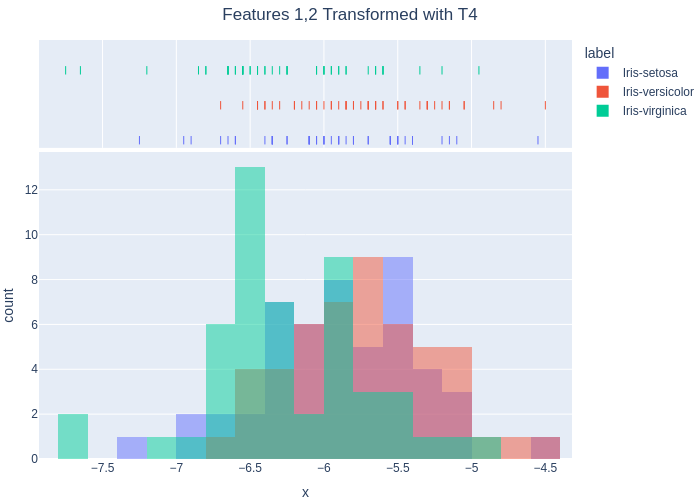
\includegraphics[width=\linewidth]{images/q3/p2/12T4.png}
    \end{subfigure}
    \hfill
    \begin{subfigure}{0.32\linewidth}
        \centering
        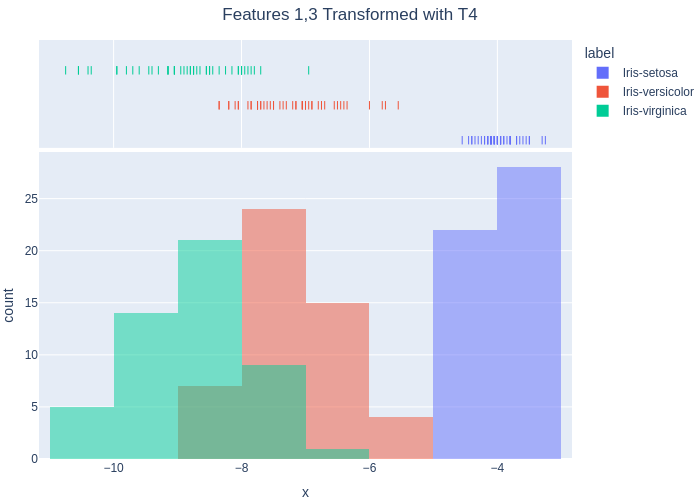
\includegraphics[width=\linewidth]{images/q3/p2/13T4.png}
    \end{subfigure}
    \hfill
    \begin{subfigure}{0.32\linewidth}
        \centering
        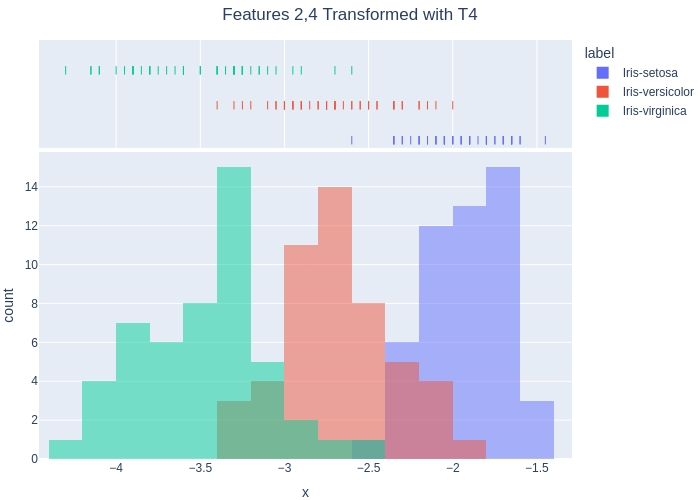
\includegraphics[width=\linewidth]{images/q3/p2/24T4.png}
    \end{subfigure}
    \caption{شکل سوال سه قسمت ب}
    \label{image-for-question1-part2}
\end{figure}

\subsection*{قسمت ج}

با توجه به اشکال رسم شده در شکل \ref{image-for-question1-part2} تبدیل‌ $T_2$ برای ویژگی‌های ۱ و ۲،
تبدیل $T_4$ برای ویژگی‌های ۱ و ۳ و همچنین برای ویژگی‌های ۲ و ۴ مناسب است. البته تبدیل
$T_3$ نیز به شکل قابل قبولی توانسته است داده‌هایی را که با استفاده از ویژگی‌های
۱ و ۳ رسم شده‌اند جدا کند. برای انتخاب بهترین ماتریس تبدیل به نمودار‌های
هیستوگرام رسم‌شده دقت می‌کنیم و ماتریس تبدیل‌هایی را که داده‌ها را به نسبت بهتر تفکیک کرده‌اند را
انتخاب می‌کنیم.

\subsection*{قسمت د}

نمودار‌های مربوط به این قسمت در شکل \ref{image-for-question1-part4} رسم شده است.

\begin{figure}[h]
    \centering
    \begin{subfigure}{0.32\linewidth}
        \centering
        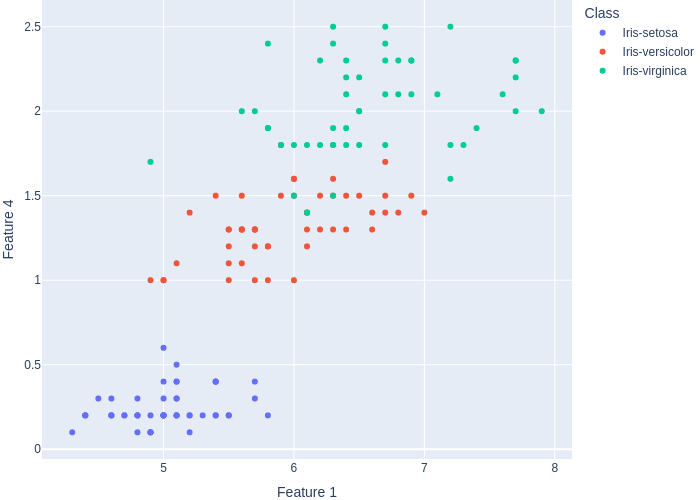
\includegraphics[width=\linewidth]{images/q3/p4/14.png}
    \end{subfigure}
    \hfill
    \begin{subfigure}{0.32\linewidth}
        \centering
        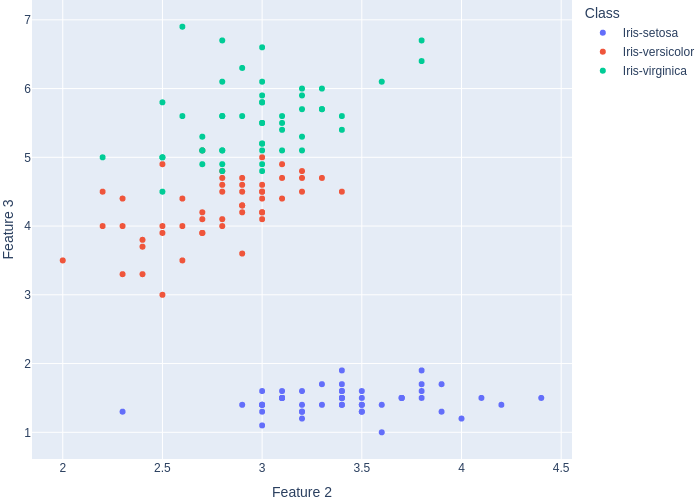
\includegraphics[width=\linewidth]{images/q3/p4/23.png}
    \end{subfigure}
    \hfill
    \begin{subfigure}{0.32\linewidth}
        \centering
        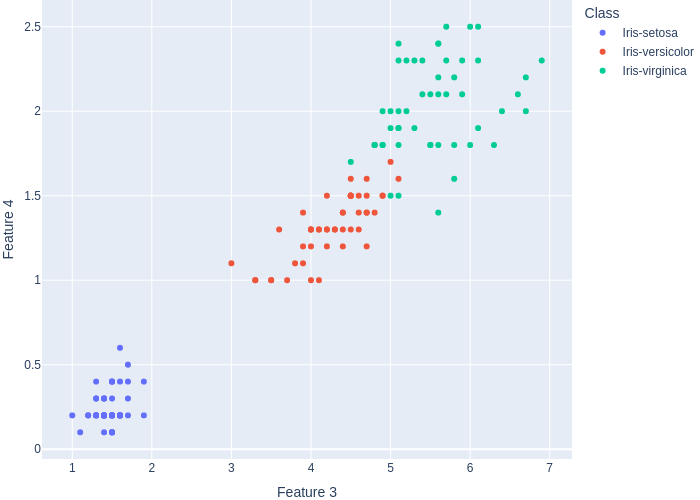
\includegraphics[width=\linewidth]{images/q3/p4/34.png}
    \end{subfigure}
    \caption{شکل سوال سه قسمت د}
    \label{image-for-question1-part4}
\end{figure}

\subsection*{قسمت ه}

نمودار توزیع‌ها پس از تبدیل با ماتریس‌های متناظر، به شکل زیر حاصل می‌شود.
(شکل \ref{image-for-question1-part5}) ماتریس تبدیل پیشنهادی
برای ویژگی‌های $(1,4)$ ماتریس $\begin{bmatrix}-0.05 \\  -1\end{bmatrix}$، ماتریس پیشنهادی برای ویژگی‌های
$(2,3)$ ماتریس $\begin{bmatrix}-0.5\\ -5\end{bmatrix}$ و ماتریس پیشنهادی برای ویژگی‌های $(3,4)$ ماتریس
$\begin{bmatrix}-2\\ -5\end{bmatrix}$ است. برای یافتن این ماتریس‌های تبدیل، از ماتریس‌های پیشنهاد شده
در قسمت‌های قبلی کمک می‌گیریم. با مقایسه‌‌ نمودار‌های حاصل از ویژگی‌هایی که در این سوال ذکر شده با نمودار‌های
حاصل از ویژگی‌هایی که در سوال‌های قبلی ذکر شده بود، متوجه می‌شویم که نمودار‌ حاصل ویژگی‌های $(1,4)$ بسیار
شبیه نمودار $(1,3)$ است. نمودار‌ مشابه $(2,3)$ نمودار $(2,4)$ و نمودار مشابه $(3,4)$ نمودار $(1,3)$
است. بر اساس سوال قبلی می‌دانیم که بهترین تبدیل برای بردار‌های متناظر این نمودار‌ها ماتریس $T_4$
است. حال ماتریس $T_4$ را به گونه‌ای برای هر یک از سه شکل تغییر می‌دهیم که تا جای ممکن گل‌ها را از
هم جدا کند.

\begin{figure}[h]
    \centering
    \begin{subfigure}{0.32\linewidth}
        \centering
        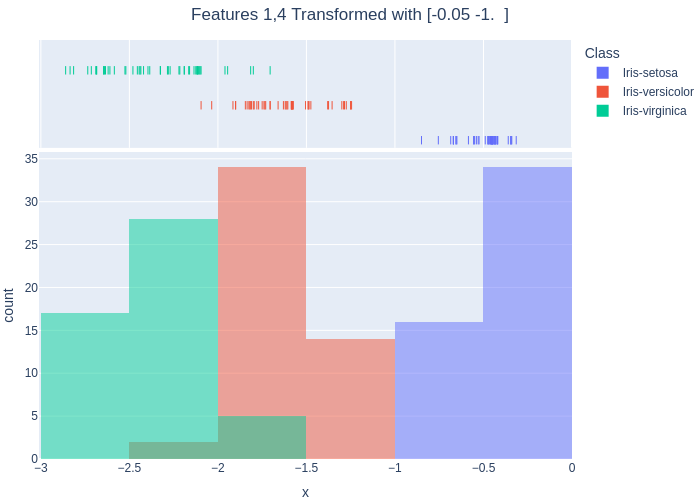
\includegraphics[width=\linewidth]{images/q3/p5/14T1.png}
    \end{subfigure}
    \hfill
    \begin{subfigure}{0.32\linewidth}
        \centering
        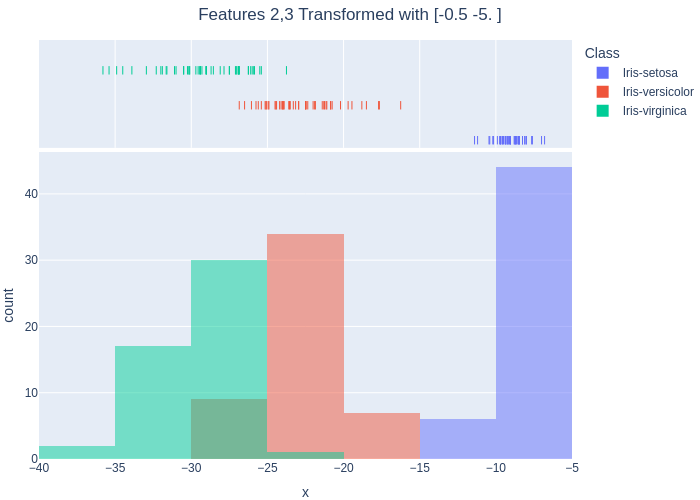
\includegraphics[width=\linewidth]{images/q3/p5/23T2.png}
    \end{subfigure}
    \hfill
    \begin{subfigure}{0.32\linewidth}
        \centering
        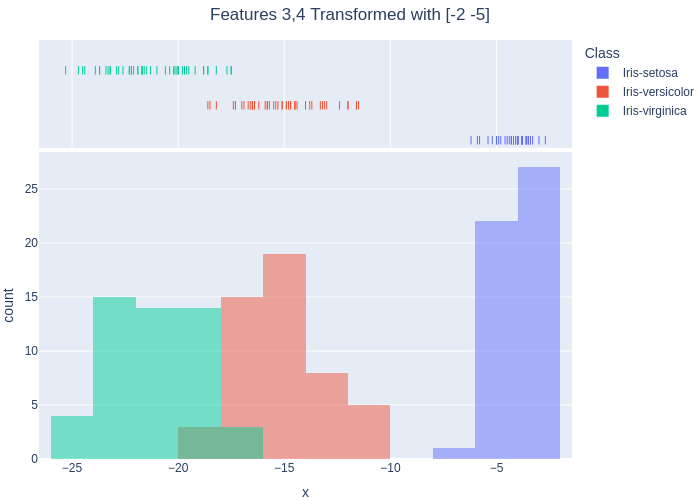
\includegraphics[width=\linewidth]{images/q3/p5/34T3.png}
    \end{subfigure}
    \caption{شکل سوال سه قسمت ه}
    \label{image-for-question1-part5}
\end{figure}

\section*{سوال چهار}

\subsection*{قسمت الف}

با توجه به درس آمار می‌دانیم اگر احتمال شکست در یک مسئله $q$ باشد، در این صورت احتمال موفقیت برابر $p=1-q$ است،
بنابراین در این مسئله از آن جا که احتمال افتادن سکه به پشت برابر $\frac{2}{3}$ است بنابراین احتمال رو افتادن سکه
$p=1 - \frac{2}{3} = \frac{1}{3}$ می‌شود. همچنین از همان درس آمار و احتمال می‌دانیم، مسئله‌ پرتاب تاس از توزیع برنولی پیروی می‌کند. از آن جا که در توزیع برنولی
با فرض  احتمال موفقیت در یک آزمایش برابر $p$، میانگین و واریانس به ترتیب برابر می‌شود با $p$ و $p(1-p)$ بنابراین در این
مسئله خواهیم داشت:‌ (۱) به طور میانگین حدود $1400\times \frac{1}{3} = 466.66$ سکه به صورت «رو»‌ می‌افتد
و (۲) انحراف معیار این فرآیند برابر $\sqrt{1400 \times \frac{1}{3}(1-\frac{1}{3})} = 17.63$ می‌شود.

\subsection*{قسمت ب}

\begin{enumerate}[label=\alph* )]
    \item  اگر هت‌تریک را به معنای حداقل سه شوت پشت سرهم موفق در نظر بگیریم، در این صورت در این مسئله باید احتمال آن که حداقل سه شوت پشت سر از شوت‌ها حتما گل شود اما شوت‌های دیگر حتما
    گل نشود را محاسبه می‌کنیم. در شکل \ref{messi-hattrick} شوت‌های گل شده با رنگ سبز و شوت‌هایی که گل نشده است با رنگ
    قرمز نشان داده شده است. برای حل مسئله مطابق شکل \ref{messi-hattrick} شوت‌هایی را که گل شده است را یک گروه در نظر گرفته
    و تعداد جایگاه‌هایی که می‌تواند قرار گیرد را محاسبه می‌کنیم.

    \begin{figure}[h]
        \centering
        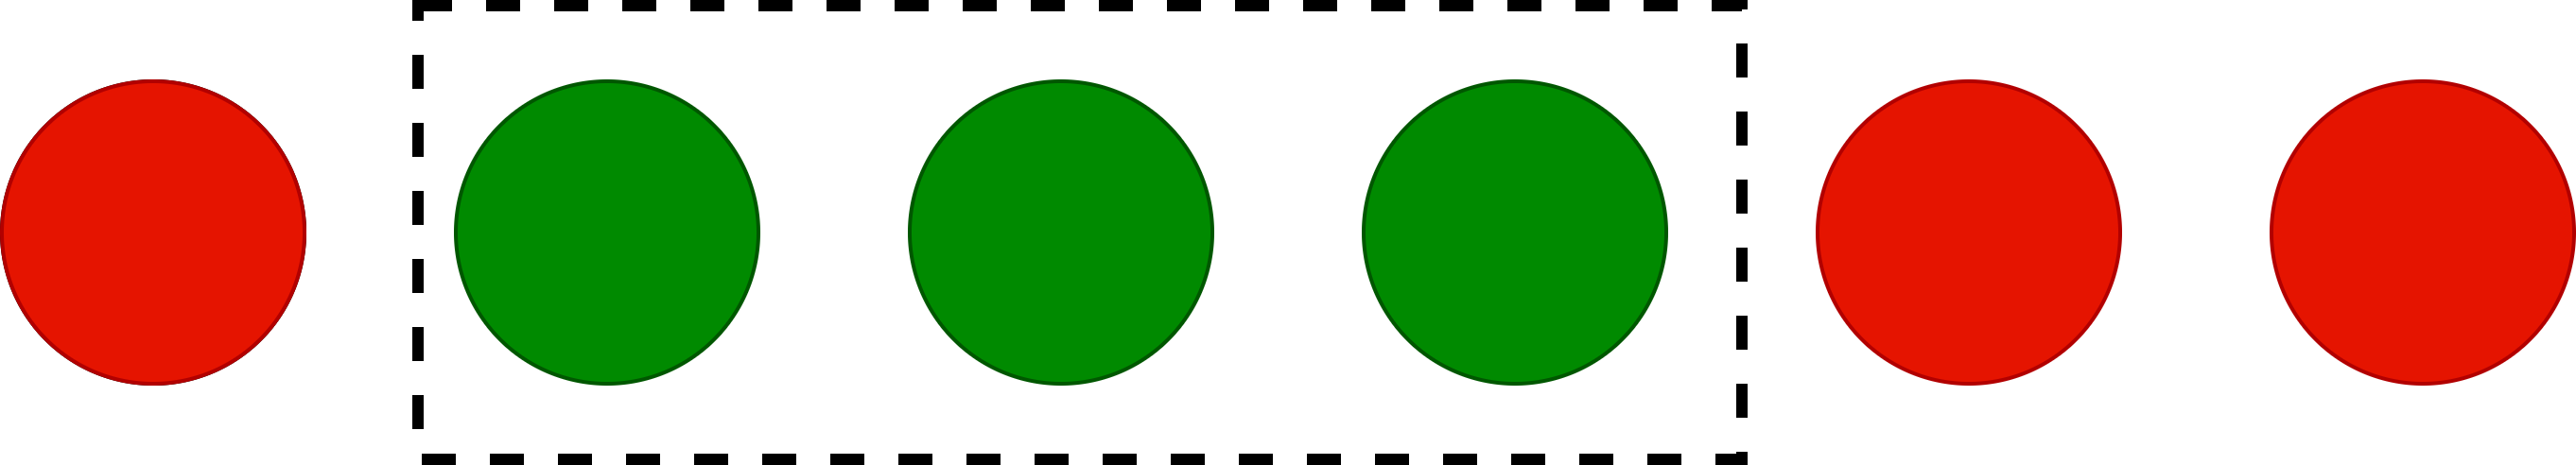
\includegraphics[width=0.5\linewidth]{images/q4/shoots.png}
        \caption{شکل مربوط به سوال ۴ قسمت ب}
        \label{messi-hattrick}
    \end{figure}

    با توجه به توضیحات بالا، احتمال این رخداد به صورت زیر محاسبه می‌شود.

    $$P(A) = \binom{4}{1} (\frac{4}{10})^3(\frac{6}{10})^3 +‌ \binom{3}{1} (\frac{4}{10})^4(\frac{6}{10})^2 +  \binom{2}{1} (\frac{4}{10})^5(\frac{6}{10})^1 + \binom{1}{1} (\frac{4}{10})^6$$

    \item با توجه به صورت سوال باید احتمال رخدادی را محاسبه کنیم که دو شوت اول گل نشود اما گل سوم
    گل شود. این احتمال به صورت زیر محاسبه می‌شود.

    $$P(B) = \frac{6}{10} \times \frac{6}{10} \times \frac{4}{10}$$
\end{enumerate}

\subsection*{قسمت ج}

برای پاسخ به این سوال ابتدا لازم است مقدار پارامتر $\lambda$ را محاسبه کنیم. برای محاسبه‌ این مقدار
از تابع توزیع پوآسن که با تابع $P(X=k)=\frac{\lambda^k e^{-\lambda}}{k!}$ بیان می‌شود استفاده می‌کنیم.

\begin{eqnarray*}
P(X=3) & = & P(X=0) + P(X=1) \\
\frac{\lambda^3 e^{-\lambda}}{3!} & = & \frac{\lambda^0 e^{-\lambda}}{0!} + \frac{\lambda^1 e^{-\lambda}}{1!} \\
\frac{\lambda^3}{3!} & = & 1 + \lambda \\
\lambda^3 - 6\lambda - 6 & = & 0
\end{eqnarray*}

با حل معادله بالا، متوجه می‌شویم که تنها ریشه $2.84732$ عدد حقیقی است، بنابراین
\linebreak
$\lambda = 2.84732$.

\begin{enumerate}[label=\alph* )]
    \item با توجه به آن که در توزیع پوآسن توزیع میانگین برابر $\lambda$ می‌شود بنابراین در این مسئله
    میانگین برابر خواهد بود با $2.84732$.
    \item در این قسمت برای ساده‌شدن محاسبات $\lambda=3$ گرفته و از جدول‌‌هایی که برای این توزیع تدارک
    دیده شده است استفاده می‌کنیم. با توجه به آن که این جداول بر مبنای توزیع تجمعی هستند، بنابراین احتمال
    داده شده را به صورت تجمعی حساب می‌کنیم.

    $$P(2 \ge X \leq 4) = P(X \leq 4) - P(X < 2) = 0.848 - 0.469 = 0.379$$
\end{enumerate}

\subsection*{قسمت د}

\begin{enumerate}[label=\alph* )]
    \item
    \begin{eqnarray*}
        E[aX+bY] & = & \frac{1}{n}\sum_{i=1}^{n} (ax_i + by_i) \\
        & = & \frac{1}{n}\sum_{i=1}^{n} ax_i + \frac{1}{n}\sum_{i=1}^{n} by_i \\
        & = & \frac{a}{n}\sum_{i=1}^{n} x_i + \frac{b}{n}\sum_{i=1}^{n} y_i \\
        & = & a(\frac{1}{n}\sum_{i=1}^{n} x_i) + b(\frac{1}{n}\sum_{i=1}^{n} y_i) \\
        & = & a E[X] + b E[Y] \\
    \end{eqnarray*}
    \item طبق تعریف واریانس داریم $E[(X-\mu_X)^2]$ بنابراین
    \begin{eqnarray*}
        \sigma_X^2 = E[(X-\mu_X)^2] & = & E[X^2 -2\mu_XX + \mu_X^2] \\
        & = & E[X^2] -2 E[\mu_XX] + E[\mu_X^2] \\
        & = & E[X^2] -2\mu_XE[X] + E[\mu_X^2] \\
        & = & E[X^2] -2\mu_X^2 + \mu_X^2 \\
        & = & E[X^2] - \mu_X^2 \\
    \end{eqnarray*}
    \item  می‌دانیم اگر دو متغیر $X$ و $Y$ از هم مستقل باشند، داریم:
    \linebreak
    $P(XY) = P(X)P(Y)$. با این دانش، ابتدا ثابت می‌کنیم اگر دو متغیر تصادفی $X$ و $Y$ از هم مستقل باشند، داریم:
    $E[XY] = E[X]E[Y]$.

    \begin{eqnarray*}
        E[XY] & = & \sum_{x}\sum_{y} xy P(X=x,Y=y) \\
        &\xrightarrow{X \; \text{\lr{and}} \;Y \;\text{\lr{are independant}}}& \sum_{x}\sum_{y} xy P(X=x)P(Y=y) \\
        &=& \big(\sum_{x}x P(X=x)\big)\big(\sum_{y} y P(Y=y)\big) \\
        &=& E[X]E[Y]
    \end{eqnarray*}

    حال به سراغ رابطه‌ $Cov(X,Y) = E[XY] - E[X]E[Y]$ می‌رویم. اندکی بالاتر اثبات کردیم که برای دو متغیر تصادفی
    $X$ و $Y$ که از هم مستقل هستند داریم: $E[XY] = E[X]E[Y]$ بنابراین خواهیم داشت $Cov(X,Y) = 0$.

    \item برای نشان دادن نقض جمله «صفر بودن همبستگی متغیر‌های تصادفی، استقلال بین آن‌ها را بیان می‌کند» از مثال
    نقض کمک می‌گیریم. نقاط روی یک دایره شعاع یک و مرکز مبدا مختصات در فضای دو بعدی را در نظر بگیرید.
    با توجه به آن که رابطه‌ی بین متغیر تصادفی $X$ و $Y$ به صورت غیرخطی و برابر $X^2 + Y^2 = 1$ است در
    نتیجه این دو متغیر مستقل از هم نیستند. حال مقدار همبستگی بین این دو متغیر تصادفی را با استفاده از
    فرمول زیر محاسبه می‌کنیم.

    $$Corr(X,Y) = \frac{E[(X-\mu_X)(Y-\mu_Y)]}{\sigma_X\sigma_Y}$$

    رابطه بالا را به شکل زیر بازنویسی می‌کنیم.

    $$Corr(X,Y) = \frac{\frac{1}{n}\sum_{x}\sum_{y} (X-\mu_X)(Y-\mu_Y)}{\sigma_X\sigma_Y}$$

    با توجه به توزیع $X$ و $Y$ داریم $\mu_X=0$ و $\mu_Y=0$. بنابراین:

    $$Corr(X,Y) = \frac{\frac{1}{n}\sum_{x}\sum_{y} XY}{\sigma_X\sigma_Y}$$

    ادعا می‌کنیم صورت مخرج برابر صفر است، چرا که در این فرمول، هر مقدار $X$ در دو مقدار $Y$ ضرب می‌شود.
    قدر مطلق این دو مقدار $Y$ با هم برابر است، اما علامت آن‌ها متفاوت است. با توجه به همین استدلال
    حاصل صورت برابر صفر می‌شود. در نتیجه $Corr(X,Y) = 0$. اما پیش‌تر رابطه‌ بین دو متغیر را بیان کرده بودیم
    در نتیجه این دو متغیر از هم مستقل نیستند. بنابراین جمله بیان شده در ابتدا نقض می‌شود.
\end{enumerate}

\section*{سوال پنج}

\subsection*{قسمت الف}

با توجه به محاسبات زیر داریم:‌ $\lambda_1 = c+d$ یا $\lambda_2 = a+b$.

\begin{eqnarray*}
    \textbf{Av} =
        \begin{bmatrix}
            a & b \\
            c & d
        \end{bmatrix}
        \begin{bmatrix}
            1 \\
            1
        \end{bmatrix} =
        \begin{bmatrix}
            a + b \\
            c + d
        \end{bmatrix} \xrightarrow[]{a+b=c+d}
        \begin{bmatrix}
            c + d \\
            c + d
        \end{bmatrix} = (c+d) \begin{bmatrix}
            1 \\
            1
        \end{bmatrix} \xrightarrow[]{a+b=c+d} (a+b) \begin{bmatrix}
            1 \\
            1
        \end{bmatrix}
\end{eqnarray*}

\subsection*{قسمت ب}

با توجه به محاسبات زیر داریم $\lambda_1 = a-c$ یا $\lambda_2 = d-b$.

\begin{eqnarray*}
    \textbf{Av} =
        \begin{bmatrix}
            a & b \\
            c & d
        \end{bmatrix}
        \begin{bmatrix}
            b \\
            -c
        \end{bmatrix} =
        \begin{bmatrix}
            ab - bc \\
            cb - cd
        \end{bmatrix}  & = &
        \begin{bmatrix}
            b\; (a-c) \\
            -c\; (d-b)
        \end{bmatrix} \\
        & \xrightarrow[\Rightarrow a-c = d-b]{a+b=c+d} &
        \begin{bmatrix}
            b\;(a-c) \\
            -c \; (a-c)
        \end{bmatrix} \\
        & = &  (a-c) \begin{bmatrix}
            b \\
            -c
        \end{bmatrix} \xrightarrow[]{a-c = d-b} (d-b) \begin{bmatrix}
            b \\
            -c
        \end{bmatrix}
\end{eqnarray*}

\subsection*{قسمت ج}

با توجه به سوال‌های قبل فضای ویژه متناظر با بردار ویژه $\begin{bmatrix}b \\ -c \end{bmatrix}$ و $\begin{bmatrix}1 \\ 1 \end{bmatrix}$
به ترتیب برابر خواهد بود با $\text{span}\{\begin{bmatrix}b \\ -c \end{bmatrix}\}$ و  $\text{span}\{\begin{bmatrix}1 \\ 1\end{bmatrix}\}$
. اگر بخواهیم مقادیر بردار‌های ویژه را با استفاده از حل مستقیم معادله بردار ویژه به دست آوریم خواهیم داشت.

سعی می‌کنیم مقادیر ویژه و بردار‌های ویژه ماتریس $\textbf{A}$ را بیابیم.

\begin{eqnarray*}
    \textbf{A}\,x & = & \lambda \, x \\
    (\textbf{A} - \lambda I) x & = & 0 \\
    |\textbf{A} - \lambda I| & = & 0 \\
    \begin{vmatrix}a-\lambda & b \\ c & d - \lambda \end{vmatrix} & = & 0 \\
    (a-\lambda)(d - \lambda) - bc & = & 0 \\
    \lambda^2 - (a+d)\lambda + ad - bc & = & 0 \\
    \lambda_1 & = & \frac{(a+d) + \sqrt{(a+d)^2-4(ad-bc)}}{2} \\
    \lambda_2 & = & \frac{(a+d) - \sqrt{(a+d)^2-4(ad-bc)}}{2} \\
\end{eqnarray*}

مقادیر لاندا حاصل می‌شود، حال به سراغ محاسبه‌ بردارهای ویژه می‌رویم.

\begin{eqnarray*}
    \textbf{A}\,x & = & \lambda \, x \\
    \begin{bmatrix}a & b\\c & d\end{bmatrix}\begin{bmatrix}e\\ f\end{bmatrix} & = & \lambda \begin{bmatrix}e\\ f\end{bmatrix} \\
    \begin{bmatrix}ae + bf\\ce + df \end{bmatrix} & = & \lambda \begin{bmatrix}e\\ f\end{bmatrix} \\
    \begin{bmatrix}ae + bf - \lambda e\\ce + df - \lambda f\end{bmatrix} & = & 0
\end{eqnarray*}

بنابراین خواهیم داشت.

\begin{eqnarray}
    \begin{cases}
        (a-\lambda)e + bf = 0 \\
        ce + (d-\lambda)f = 0
    \end{cases}
\end{eqnarray}

با حل معادله (۱) داریم: $f = \frac{\lambda - a}{b} e$. با جایگذاری مقادیر ویژه در این بردار‌ها خواهیم داشت.

\begin{eqnarray*}
    \textbf{v}_1 = \begin{bmatrix}1\\ \frac{\lambda_1 - a}{b}\end{bmatrix} \hspace{1cm} \textbf{v}_1 = \begin{bmatrix}1\\ \frac{\lambda_2 - a}{b}\end{bmatrix}
\end{eqnarray*}

اگر مقدار $b=0$ اما $c\neq 0$ باشد در این صورت معادله‌ (۱) را به صورت زیر حل می‌کنیم. $e = \frac{d-\lambda}{c}f$
بنابراین بردار‌های ویژه به شکل زیر حاصل می‌شود.

\begin{eqnarray*}
    \textbf{v}_1 = \begin{bmatrix}1\\ \frac{d - \lambda_1}{c}\end{bmatrix} \hspace{1cm} \textbf{v}_1 = \begin{bmatrix}1\\ \frac{d - \lambda_2}{c}\end{bmatrix}
\end{eqnarray*}

اما اگر $c=0, b=0$ باشد در این صورت باید بردار‌های ویژه را به طریق دیگری به دست بیاوریم. ابتدا مقادیر ویژه را
به شکل زیر حساب می‌کنیم.

\begin{eqnarray*}
    \lambda_1 & = & \frac{(a+d) + \sqrt{(a+d)^2-4ad}}{2} = \frac{(a+d) + |a-d|}{2} \\
    \lambda_2 & = & \frac{(a+d) - \sqrt{(a+d)^2-4ad}}{2} = \frac{(a+d) - |a-d|}{2}\\
\end{eqnarray*}

اگر $a \neq d$ باشد، خواهیم داشت $\lambda_1 = a, \lambda_2=d$. بردار‌های ویژه متناظر این مقادیر ویژه
با توجه به معادله‌ (۱) برابر خواهد بود با

\begin{eqnarray*}
    \textbf{v}_1 = \begin{bmatrix}1\\ 0\end{bmatrix} \hspace{1cm} \textbf{v}_2 = \begin{bmatrix}0\\ 1\end{bmatrix}
\end{eqnarray*}

\subsection*{قسمت د}

با توجه به دانسته‌های حاصل از قسمت‌های قبلی سوال، داریم.

\begin{align*}
    \lambda_1 = 0.75 + 0.25 = 1  & \hspace{3cm}
    \boldsymbol{v_1} = \begin{bmatrix}
            1 \\
            1
        \end{bmatrix}
    \\
    \lambda_2  =   0.75 - 0.25 = 0.5  & \hspace{3cm}
    \boldsymbol{v_2} = \begin{bmatrix}
            0.25 \\
            -0.25
        \end{bmatrix}
\end{align*}

\subsection*{قسمت ه}

خواهیم داشت.

\begin{eqnarray*}
    \textbf{A}\overrightarrow{d_*} & = & \overrightarrow{d_*}\\
    \begin{bmatrix}0.75 & 0.25\\ 0.25 & 0.75\end{bmatrix}\overrightarrow{d_*} & = & \overrightarrow{d_*} \\
    \begin{bmatrix}0.75 & 0.25\\ 0.25 & 0.75\end{bmatrix}\begin{bmatrix}x\\ y\end{bmatrix} & = & \begin{bmatrix}x\\ y\end{bmatrix} \\
    \begin{bmatrix}0.75x+0.25y\\ 0.25x+0.75y\end{bmatrix} & = & \begin{bmatrix}x\\ y\end{bmatrix} \\
    \begin{bmatrix}-0.25x+0.25y\\ 0.25x-0.25y\end{bmatrix} & = & \begin{bmatrix}0\\ 0\end{bmatrix}
\end{eqnarray*}

بنابراین

\begin{eqnarray*}
    \begin{cases} -0.25x+0.25y = 0 \\ 0.25x-0.25y = 0\end{cases} \Longrightarrow x = y
\end{eqnarray*}

با توجه به محاسبات بالا، به ازای تمامی $\overrightarrow{d_*}=\begin{bmatrix}x\\y\end{bmatrix}$
ها که $x=y$ است خواهیم داشت
\break
$\textbf{A}\overrightarrow{d_*} = \overrightarrow{d_*}$.

\subsection*{قسمت و}

با توجه به قسمت‌های قبلی می‌دانیم که بردار $\begin{bmatrix}
    1 \\
    -1
\end{bmatrix}$ جزو بردار‌های ویژه ماتریس $\textbf{A}$ است. همچنین می‌دانیم مقدار ویژه متناظر این بردار $0.5$ است.
در نتیجه با ضرب ماتریس $\textbf{A}$ در این ماتریس حاصل برابر خواهد بود با $0.5 \begin{bmatrix}
    1 \\
    -1
\end{bmatrix}$ بدین معنی که از شدت علاقه خسرو و تنفر شیرین کاسته می‌شود.
حال اگر ماتریس $\textbf{A}$
را بی نهایت بار را در این بردار ضرب کنیم، حاصل برابر خواهد بود با $(0.5)^n \begin{bmatrix}
    1 \\
    -1
\end{bmatrix}$ همان‌طور که ملاحظه می‌شود با زیاد شدن $n$ بزرگی ماتریس رفته‌رفته کم‌تر می‌شود. بدین معنی که
از عشق خسرو و نفرت شیرین رفته‌رفته کاسته شده و روابط میان‌ آن‌ها معمولی می‌شود.

\subsection*{قسمت ز}

بردار داده شده را با استفاده بردار‌های ویژه ماتریس بازنویسی می‌کنیم.

\begin{align*}
    a \begin{bmatrix}1 \\ 1\end{bmatrix} + b \begin{bmatrix}1\\ -1\end{bmatrix} & = \begin{bmatrix}3\\ 5\end{bmatrix} \\
    \begin{bmatrix}a + b \\ a - b\end{bmatrix} & = \begin{bmatrix}3\\ 5\end{bmatrix}
\end{align*}

با حل دستگاه بالا داریم $a=4, b=-1$. حال به سراغ محاسبه‌ی سرنوشت عشق میان خسرو و شیرین با استفاده از بردار داده شده
می‌رویم.

\begin{align*}
    \lim_{n \to \infty} \boldsymbol{A}^n\Big(4 \begin{bmatrix}1 \\ 1\end{bmatrix} - \begin{bmatrix}1\\ -1\end{bmatrix}\Big) & =
    \lim_{n \to \infty} \boldsymbol{A}^{n-1}\Big(4 (\boldsymbol{A}\begin{bmatrix}1 \\ 1\end{bmatrix}) - (\boldsymbol{A} \begin{bmatrix}1\\ -1\end{bmatrix}) \Big) \\
    & = \lim_{n \to \infty} \boldsymbol{A}^{n-1}\Big(4 (1\begin{bmatrix}1 \\ 1\end{bmatrix}) - (0.5\begin{bmatrix}1\\ -1\end{bmatrix}) \Big) \\
    & = \lim_{n \to \infty} \Big(4 (1^n\begin{bmatrix}1 \\ 1\end{bmatrix}) - (0.5^{n}\begin{bmatrix}1\\ -1\end{bmatrix}) \Big) \\
    & = 4 \begin{bmatrix}1 \\ 1\end{bmatrix} = \begin{bmatrix}4 \\ 4\end{bmatrix}
\end{align*}

با توجه محاسبات بالا در نهایت یک واحد از عشق خسرو کم شده و به عشق شیرین اضافه می‌شود.

\subsection*{قسمت ح}

مشابه روال قبل داریم.

\begin{align*}
    \lambda_1 = 1 + 1 = 2  & \hspace{3cm} \boldsymbol{v_1} = \begin{bmatrix} 1 \\ 1 \end{bmatrix}
    \\
    \lambda_2  =  1 - 1 = 0  & \hspace{3cm} \boldsymbol{v_2} = \begin{bmatrix} 1 \\ -1\end{bmatrix}
\end{align*}

\subsection*{قسمت ط}

با توجه به محاسبات زیر پس از طی یک دوره صفر می‌شود. با روندی مشابه در بی‌نهایت نیز صفر می‌شود.

\begin{align*}
     \boldsymbol{A} \begin{bmatrix}1 \\ -1\end{bmatrix} = 0 \times \begin{bmatrix}1 \\ -1\end{bmatrix} = \begin{bmatrix}0 \\ 0\end{bmatrix}
\end{align*}

\subsection*{قسمت ی}

بر طبق محاسبات زیر، عشق آن‌ها نسبت به یکدیگر دو برابر می‌شود.

\begin{align*}
    \boldsymbol{A}\begin{bmatrix}1 \\ 1\end{bmatrix} & = 2\begin{bmatrix}1 \\ 1\end{bmatrix}
\end{align*}

در بی‌نهایت نیز عشق خسرو نسبت به شیرین و بالعکس به بی‌نهایت میل می‌کند، چرا که.

\begin{align*}
    \lim_{n \to \infty} \boldsymbol{A}^n\begin{bmatrix}1 \\ 1\end{bmatrix} & =
    \lim_{n \to \infty} \boldsymbol{A}^{n-1} (\boldsymbol{A}\begin{bmatrix}1 \\ 1\end{bmatrix})\\
    & = \lim_{n \to \infty} \boldsymbol{A}^{n-1} (2\begin{bmatrix}1 \\ 1\end{bmatrix}) \\
    & = \lim_{n \to \infty} 2^n\begin{bmatrix}1 \\ 1\end{bmatrix} \\
    & = \begin{bmatrix}\infty \\ \infty\end{bmatrix} \\
\end{align*}

\subsection*{قسمت ک}

داریم.

\begin{align*}
    \lambda_1 = 1 - 2 = -1  & \hspace{3cm} \boldsymbol{v_1} = \begin{bmatrix} 1 \\ 1 \end{bmatrix}
    \\
    \lambda_2  =  1 - (-2) = 3  & \hspace{3cm} \boldsymbol{v_2} = \begin{bmatrix} -2 \\ 2\end{bmatrix}
\end{align*}

\subsection*{قسمت ل}

با توجه به محاسبات زیر در ابتدا خسرو شیرین را دوست دارد و رفته‌رفته این علاقه بیشتر می‌شود
اما شیرین از ابتدا خسرو را دوست ندارد و رفته‌رفته تنفر او از خسرو بیشتر می‌شود.

\begin{align*}
    \boldsymbol{A}^n \begin{bmatrix} -1 \\ 1 \end{bmatrix} & = \boldsymbol{A}^{n-1} \Bigl(\boldsymbol{A}\begin{bmatrix} -1 \\ 1 \end{bmatrix}\Bigr) \\
     & = \boldsymbol{A}^{n-1} \Bigl(3\begin{bmatrix} -1 \\ 1 \end{bmatrix}\Bigr) \\
     & = 3^{n}\begin{bmatrix} -1 \\ 1 \end{bmatrix}
\end{align*}

\subsection*{قسمت م}

با توجه به محاسبات زیر، بزرگی (عشق/تنفر) آن‌ها در طول زمان تغییری نمی‌کند اما در روز‌های زوج
آن‌ها عاشق یکدیگرند ولی در روز‌های فرد از هم متنفرند.

\begin{align*}
    \boldsymbol{A}^n \begin{bmatrix} 1 \\ 1 \end{bmatrix} & = \boldsymbol{A}^{n-1} \Bigl(\boldsymbol{A}\begin{bmatrix} 1 \\ 1 \end{bmatrix}\Bigr) \\
     & = \boldsymbol{A}^{n-1} \Bigl((-1)\begin{bmatrix} 1 \\ 1 \end{bmatrix}\Bigr) \\
     & = (-1)^{n}\begin{bmatrix} 1 \\ 1 \end{bmatrix} \\
     & = \begin{cases}
            \begin{bmatrix} 1 \\ 1 \end{bmatrix} &\quad n \; \text{mod} \; 2 = 0\\
            \\
            \begin{bmatrix} -1 \\ -1 \end{bmatrix} &\quad n \; \text{mod} \; 2 = 1\\
        \end{cases}
\end{align*}

\section*{سوال شش}

\subsection*{قسمت الف}

نمودار به شکل \ref{table-and-plot-of-the-mean-location} حاصل می‌شود.

\begin{figure}[h]
    \begin{subfigure}{0.3\linewidth}
        \centering
        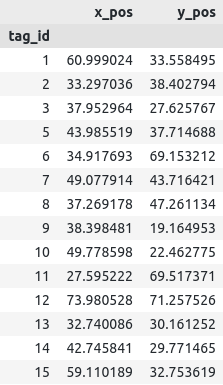
\includegraphics[scale=0.25]{images/q6/parta/table.png}
        \caption{جدول موقعیت میانگین هر بازیکن}
    \end{subfigure}
    \hfill
    \begin{subfigure}{0.65\linewidth}
        \centering
        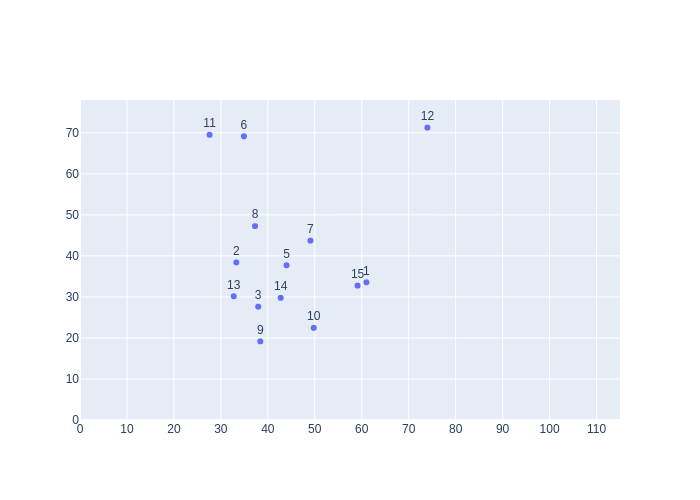
\includegraphics[scale=0.3]{images/q6/parta/scatter.png}
        \caption{جدول موقعیت میانگین هر بازیکن}
    \end{subfigure}
    \caption{شکل قسمت الف سوال شش}
    \label{table-and-plot-of-the-mean-location}
\end{figure}

\subsection*{قسمت ب}

نمودار‌های خواسته شده به شکل زیر حاصل می‌شود. (شکل \ref{normal-distribution-of-the-players-in-the-game})
کواریانس و میانگین مربوط به مختصات هر یک از بازیکنان در نمودار متناظر آن‌ها آمده است.

\begin{figure}[h]
    \centering
    \begin{subfigure}{0.3\linewidth}
        \centering
        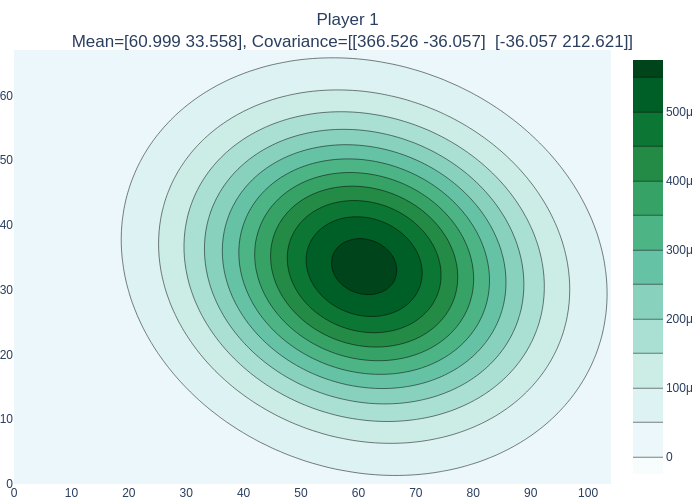
\includegraphics[scale=0.1]{images/q6/partb/1.png}
    \end{subfigure}
    \hfill
    \begin{subfigure}{0.3\linewidth}
        \centering
        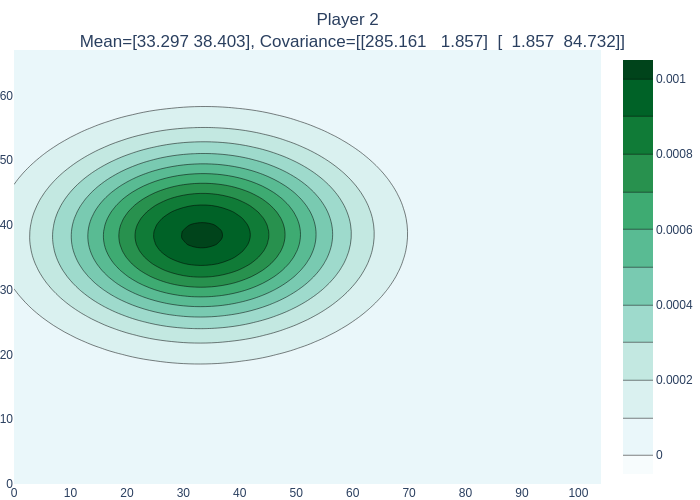
\includegraphics[scale=0.1]{images/q6/partb/2.png}
    \end{subfigure}
    \hfill
    \begin{subfigure}{0.3\linewidth}
        \centering
        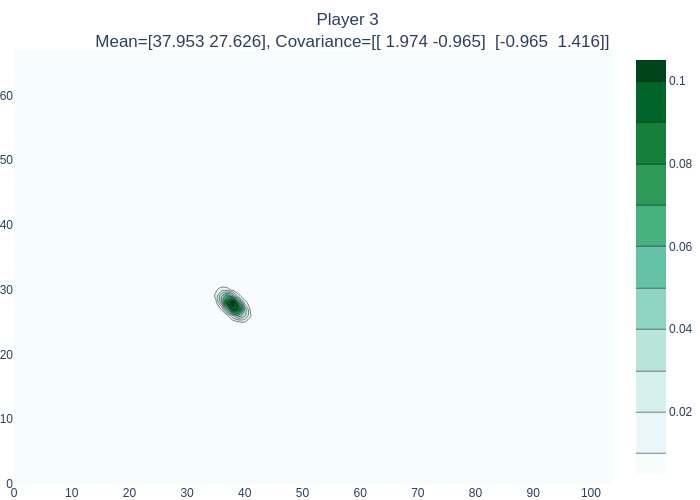
\includegraphics[scale=0.1]{images/q6/partb/3.png}
    \end{subfigure}
    \newline
    \begin{subfigure}{0.3\linewidth}
        \centering
        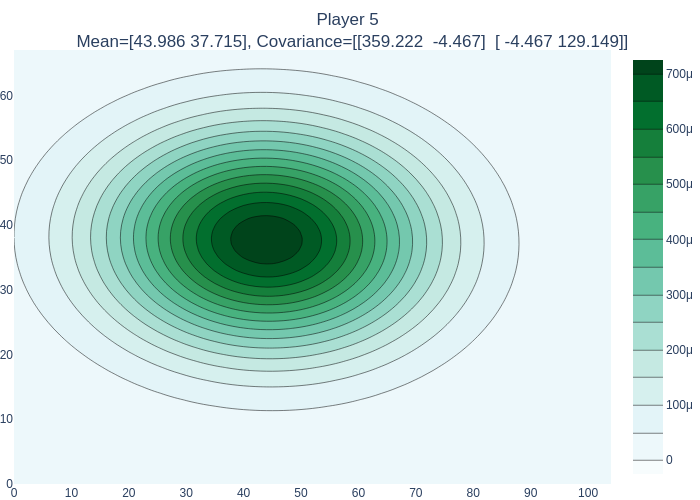
\includegraphics[scale=0.1]{images/q6/partb/5.png}
    \end{subfigure}
    \hfill
    \begin{subfigure}{0.3\linewidth}
        \centering
        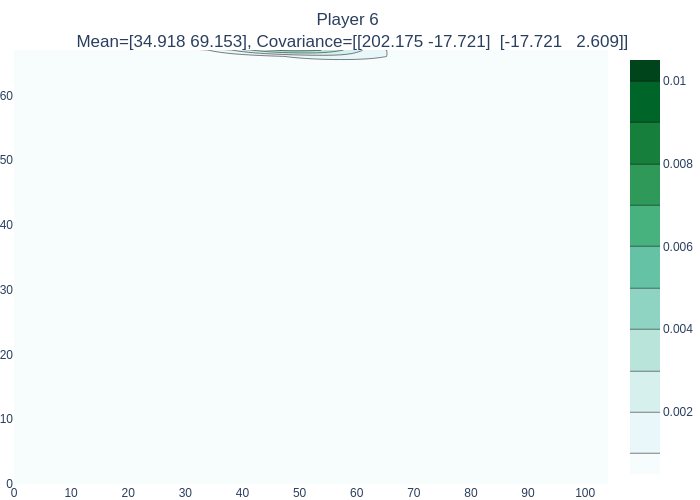
\includegraphics[scale=0.1]{images/q6/partb/6.png}
    \end{subfigure}
    \hfill
    \begin{subfigure}{0.3\linewidth}
        \centering
        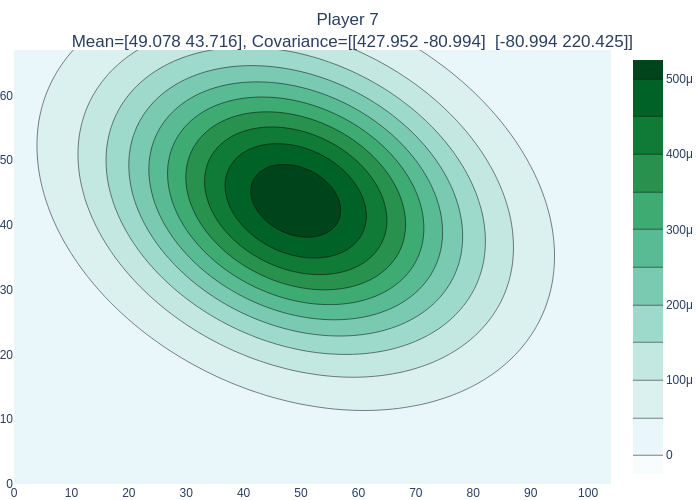
\includegraphics[scale=0.1]{images/q6/partb/7.png}
    \end{subfigure}
    \newline
    \begin{subfigure}{0.3\linewidth}
        \centering
        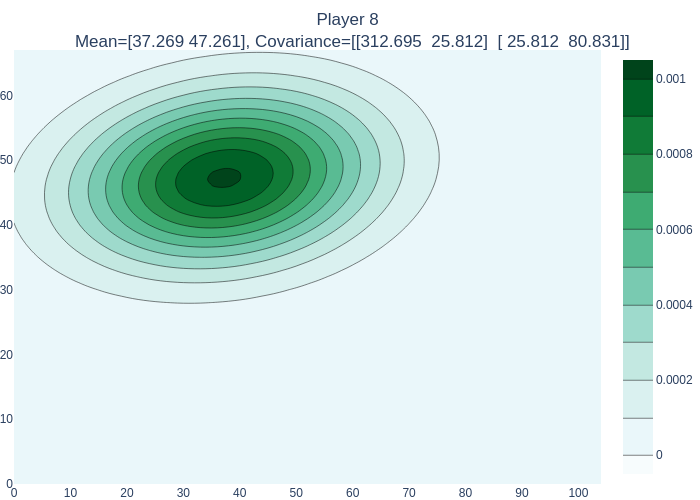
\includegraphics[scale=0.1]{images/q6/partb/8.png}
    \end{subfigure}
    \hfill
    \begin{subfigure}{0.3\linewidth}
        \centering
        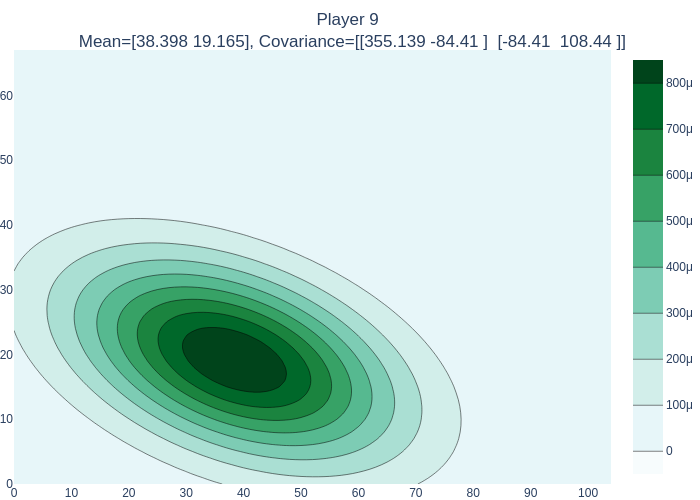
\includegraphics[scale=0.1]{images/q6/partb/9.png}
    \end{subfigure}
    \hfill
    \begin{subfigure}{0.3\linewidth}
        \centering
        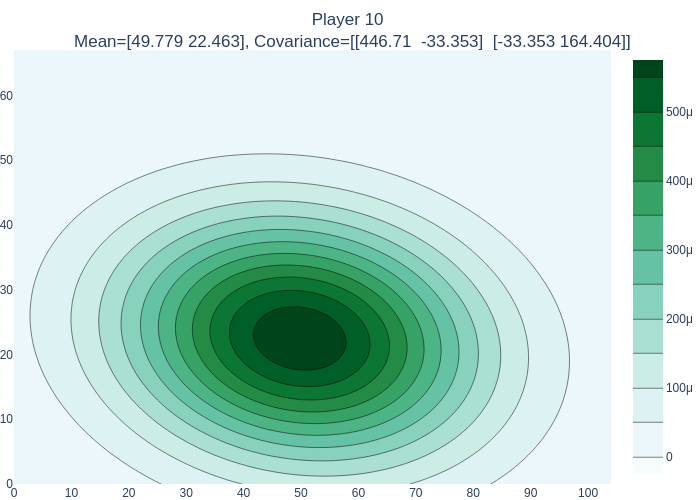
\includegraphics[scale=0.1]{images/q6/partb/10.png}
    \end{subfigure}
    \newline
    \begin{subfigure}{0.3\linewidth}
        \centering
        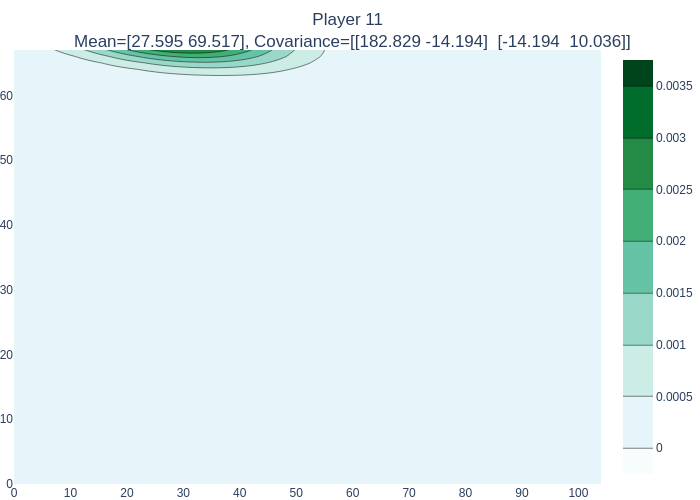
\includegraphics[scale=0.1]{images/q6/partb/11.png}
    \end{subfigure}
    \hfill
    \begin{subfigure}{0.3\linewidth}
        \centering
        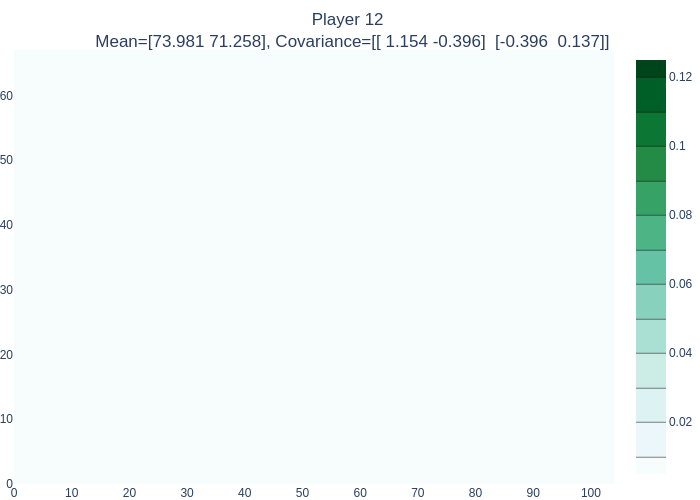
\includegraphics[scale=0.1]{images/q6/partb/12.png}
    \end{subfigure}
    \hfill
    \begin{subfigure}{0.3\linewidth}
        \centering
        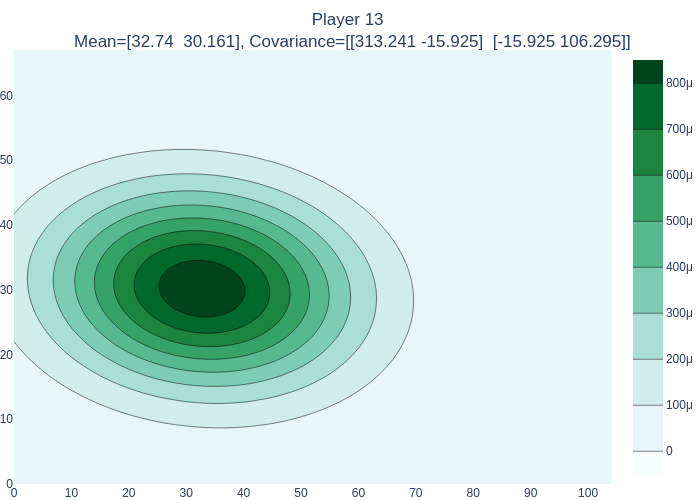
\includegraphics[scale=0.1]{images/q6/partb/13.png}
    \end{subfigure}
    \newline
    \hfill
    \begin{subfigure}{0.3\linewidth}
        \centering
        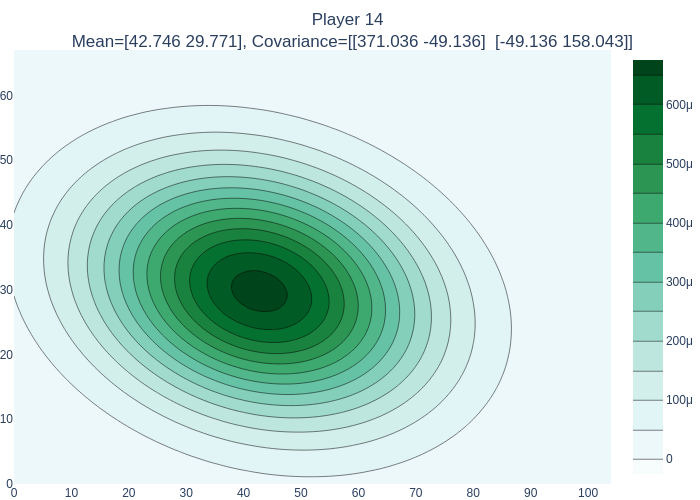
\includegraphics[scale=0.1]{images/q6/partb/14.png}
    \end{subfigure}
    \hfill
    \begin{subfigure}{0.3\linewidth}
        \centering
        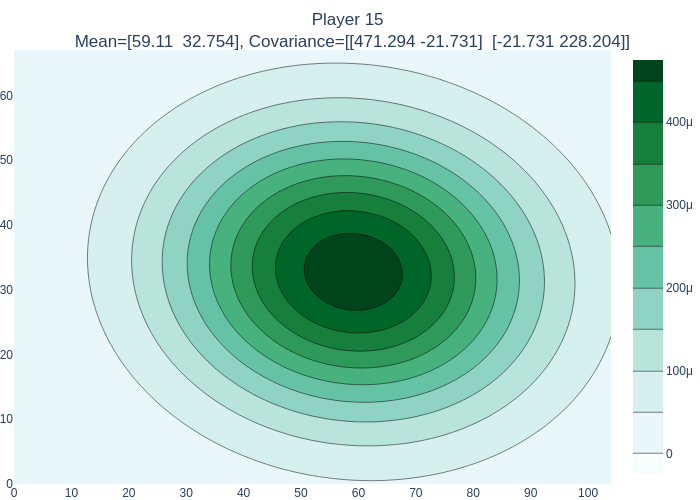
\includegraphics[scale=0.1]{images/q6/partb/15.png}
    \end{subfigure}
    \hfill
    \caption{شکل قسمت ب سوال هشت}
    \label{normal-distribution-of-the-players-in-the-game}
\end{figure}

\subsection*{قسمت ج}

نتایج به صورت زیر حاصل شده است. (شکل \ref{randomly-selected-players-and-corresponding-probability})

\begin{figure}[h]
    \centering
    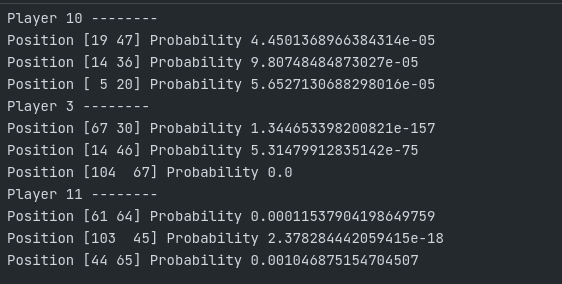
\includegraphics[scale=0.25]{images/q6/partc.png}
    \caption{شکل قسمت ج سوال هشت}
    \label{randomly-selected-players-and-corresponding-probability}
\end{figure}

\subsection*{قسمت د}

در جدول \ref{role-of-the-players} اطلاعات مربوط آمده است.

\begin{table}[h]
    \centering
    \caption{نقش‌های بازیکنانی که در دیتاست آورده شده‌اند.}
    \label{role-of-the-players}
    \begin{tabular}{c|c}
        شماره بازیکن & نقش \\
        \hline
        1 & مهاجم\\
        2 & دفاع وسط\\
        3 & مشخص نیست\\
        4 & -\\
        5 & هافبک وسط\\
        6 & ذخیره\\
        7 & هافبک چپ\\
        8 & دفاع سمت چپ \\
        9 & دفاع سمت راست\\
        10 & هافبک سمت راست\\
        11 & ذخیره\\
        12 & ذخیره\\
        13 & دفاع وسط\\
        14 & هافبک وسط\\
        15 & مهاجم
    \end{tabular}
\end{table}

\section*{سوال هفت}

\subsection*{قسمت الف}

تبدیل \lr{whitening} برای از بین بردن همبستگی میان داده‌ها استفاده می‌شود. یعنی اگر پیش از اعمال تبدیل،
همبستگی بین ویژگی‌ها برابر $\Sigma$ باشد، پس از این تبدیل ماتریس همبستگی به ماتریس همانی یا $I$ تبدیل می‌شود.
صفر شدن همبستگی بین متغیر‌ها باعث می‌شود، با استفاده از همان ویژگی‌ها مدل بهتری بر روی داده‌ها آموزش ببیند.
به همین دلیل این تبدیل را در مرحله‌ پیش‌پردازش اعمال می‌کنند.

\subsection*{قسمت ب}

این نظر را این گونه می‌توان توجیه کرد که در مسائل دسته‌بندی تعداد کلاس‌ها به صورت گسسته است. در صورتی که
در مسائل رگرسیون تعداد کلاس‌ها پیوسته است. از آن جا که در اکثر مسائل، مانند عملگر سیگما و انتگرال،
حالت‌های گسسته حالت خاصی از پیوسته است در نتیجه در این جا نیز چنین چیزی قابل عنوان است.

\subsection*{قسمت ج}

اگر $T$ یک تبدیل  خطی از یک زیرفضای $F$ در فضای برداری $V$ به همان فضای برداری باشد و $\textbf{v}$ یک بردار غیرصفر باشد
آنگاه $\textbf{v}$ یک بردار ویژه برای تبدیل $T$ است اگر

$$T(\textbf{v}) = \lambda \textbf{v}$$

در رابطه‌ی بالا مقدار $\lambda$ یک مقدار ثابت است که مقدار ویژه بردار $\textbf{v}$ نامیده می‌شود.

\subsection*{قسمت د}

اگر $\textbf{M}$ یک تبدیل خطی بوده و بردار $\textbf{v}$ بردار ویژه ماتریس باشد، در این صورت با محاسبه‌
تبدیل بردار $\textbf{v}$ با ماتریس $\textbf{M}$ بردار $\textbf{v}$ در همان جهت باقی می‌ماند اما از لحاظ
بزرگی در یک عدد ثابت($\lambda$) ضرب می‌شود. این بیان در شکل \ref{eigenvalue-and-eigenvector-interpretation}
نیز دیده می‌شود.

\begin{figure}[h]
    \centering
    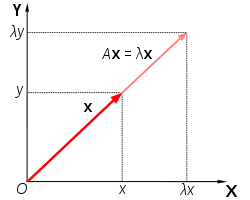
\includegraphics[scale=0.4]{images/q7/250px-Eigenvalue_equation.svg.png}
    \caption{تفسیر بردار ویژه و مقدار ویژه}
    \label{eigenvalue-and-eigenvector-interpretation}
\end{figure}

\subsection*{قسمت ه}

برای رنک‌کردن وبسایت‌های موجود در اینترنت به ماتریس $\textbf{A}$ و بردار $v$ نیازمندیم.  $a_{i,j}$ به شرطی
برابر یک است که وبسایت $j$ام به وبسایت $i$ام لینک داده باشد. به علاوه هر ستون ماتریس $\textbf{A}$
با تقسیم بر اندازه بردار آن ستون، دارای اندازه واحد شده است. بردار $v$ نیز برداری است که تمامی درایه‌های
آن برابر یک است. برای به دست آوردن اعتبار تمامی وبسایت‌های موجود در اینترنت،
ماتریس $\textbf{A}$ را در $\textbf{v}$ ضرب کرده و حاصل را با مقدار ماتریس $\textbf{A}$ جایگزین کرده
و مجددا ماتریس $\textbf{A}$ جدید را در $\textbf{v}$ ضرب می‌کنیم. این عمل را آن‌قدر تکرار می‌کنیم که
با ضرب ماتریس $\textbf{A}$ و $\textbf{v}$ ماتریس حاصل شده تغییر چندانی با ماتریس $\textbf{A}$
نکند.

با توجه به مطالب موجود در اینترنت\LTRfootnote{\lr{https://setosa.io/ev/eigenvectors-and-eigenvalues/}}
به جای روند بالا که روند زمان‌بر و کندی است، می‌توانیم مقادیر ویژه ماتریس $\textbf{A}$ را حساب کرده و
با استفاده از آن‌ها ماتریس $\textbf{A}$ بهینه را به دست بیاریم. علت این کار آن است که همان‌طور که در شکل
\ref{eigen-process} دیده می‌شود با ضرب‌های  مکرر ماتریس $\textbf{A}$ در $\textbf{v}$ حاصل به سمت بردار‌های ویژه $\textbf{A}$
کشیده می‌شود. با به دست آوردن این بردار‌ها بهتر می‌توان رفتار این ضرب را در بی‌نهایت بررسی کرد.

\begin{figure}[h]
    \centering
    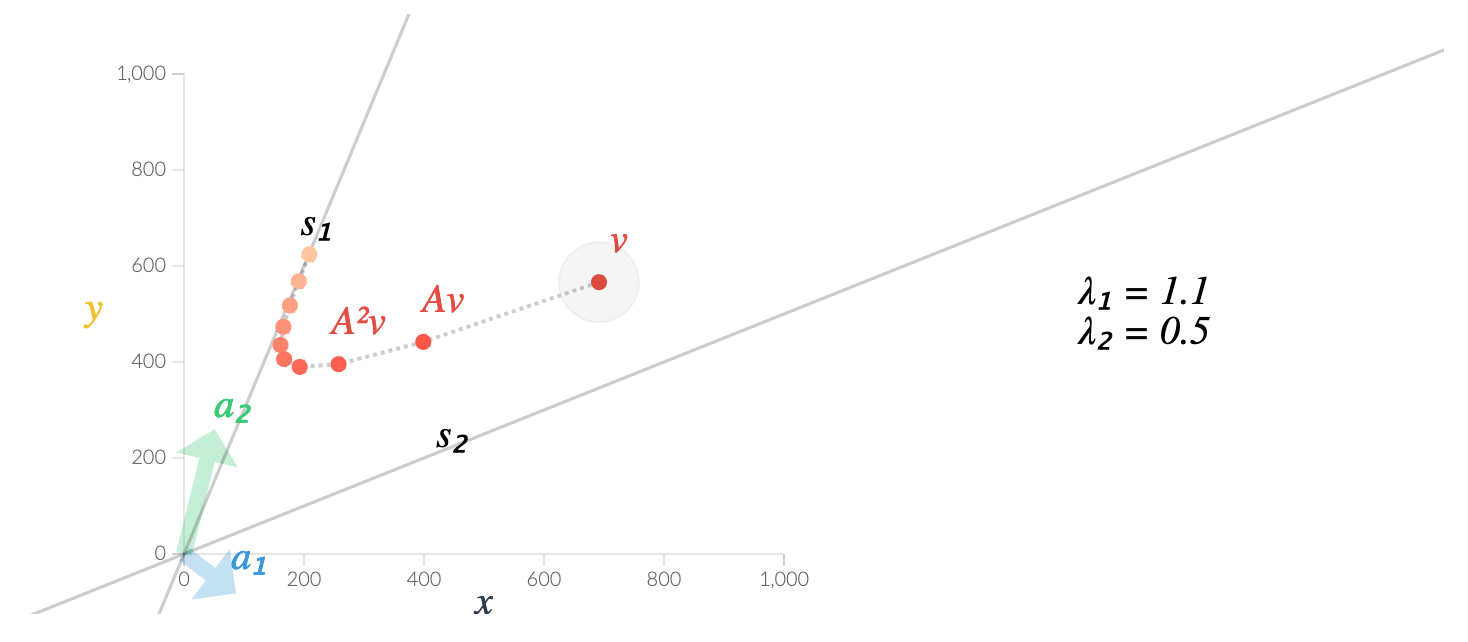
\includegraphics[scale=0.4]{images/q7/eigen_process.png}
    \caption{با ضرب مکرر $\textbf{A}$ در $\textbf{v}$ حاصل به سمت بردار‌های ویژه ماتریس $\textbf{A}$ می‌رود}
    \label{eigen-process}
\end{figure}

\end{document}